\documentclass[french, 11pt]{article}
\usepackage[utf8]{inputenc}
\usepackage[T1]{fontenc}
\usepackage{lmodern}
\usepackage{babel}
\usepackage{csquotes}
\pagestyle{empty}
\usepackage{soul}
\usepackage{setspace}
\usepackage{epigraph}
\usepackage{microtype}
\usepackage{xurl}
\usepackage{adjustbox}
\usepackage{float}
\usepackage{newtxtext,newtxmath}
\usepackage{helvet}

% Souligne le segment avec la couleur du mode et trace une flèche
% pointant vers la catégorie émotionnelle exprimée.
\newcommand{\modeAnnot}[3]{%
  % #1 = couleur du mode, #2 = segment textuel, #3 = émotion exprimée
  \begin{tikzpicture}[baseline=(T.base)]
    \node[inner sep=1pt] (T)
      {\begingroup\setulcolor{#1}\ul{#2}\endgroup};
    \node[below=8pt of T.south, anchor=north,
          font=\scriptsize\itshape, text=#1] (E) {#3};
    \draw[-{Stealth[length=3pt, width=2.5pt]}, #1]
      (T.south) -- (E.north);
  \end{tikzpicture}%
}
\newcommand{\mDesigne}[2]{\modeAnnot{colDesigne}{#1}{#2}}
\newcommand{\mComp}[2]{\modeAnnot{colComp}{#1}{#2}}
\newcommand{\mSugg}[2]{\modeAnnot{colSugg}{#1}{#2}}
\newcommand{\mMontre}[2]{\modeAnnot{colMontre}{#1}{#2}}
% =====================================================================

% --- Mathématiques ---
\usepackage{amsmath, amssymb, stmaryrd}

% --- TikZ ---
\usepackage{tikz}
\usetikzlibrary{calc, positioning, arrows.meta, shapes.geometric, shadows,
                decorations.pathreplacing, fit, backgrounds, matrix,
                babel}

% --- Mise en page ---
\usepackage{geometry}
\usepackage{xcolor}
\usepackage{array, booktabs}
\usepackage{enumitem}

% =====================================================================
%  COULEURS
% =====================================================================

% Couleurs utilitaires
\definecolor{mycyan}{RGB}{0, 170, 210}
\definecolor{mygreen}{RGB}{0, 150, 80}
\definecolor{myorange}{RGB}{210, 120, 20}
\definecolor{myred}{RGB}{190, 50, 50}
\definecolor{mygrey}{RGB}{100, 100, 100}
\definecolor{bleufonce}{RGB}{30, 60, 110}

% --- Couleurs pour les 4 modes d'expression ---
\definecolor{colDesigne}{RGB}{40, 80, 160}    % Bleu    — Explicite, direct
\definecolor{colComp}{RGB}{0, 130, 100}       % Teal    — Physiologique, organique
\definecolor{colSugg}{RGB}{180, 100, 20}      % Ambre   — Inférence, situation
\definecolor{colMontre}{RGB}{120, 50, 140}    % Violet  — Formel, stylistique

% =====================================================================
%  COMMANDES – MODES D'EXPRESSION
% =====================================================================

% ---- Soulignement coloré (soul) ----
\newcommand{\ulDesigne}[1]{\begingroup\setulcolor{colDesigne}\ul{#1}\endgroup}
\newcommand{\ulComp}[1]{\begingroup\setulcolor{colComp}\ul{#1}\endgroup}
\newcommand{\ulSugg}[1]{\begingroup\setulcolor{colSugg}\ul{#1}\endgroup}
\newcommand{\ulMontre}[1]{\begingroup\setulcolor{colMontre}\ul{#1}\endgroup}

% ---- Encadrement coloré (fcolorbox) – pour segments courts ----
\newcommand{\fboxDesigne}[1]{\fcolorbox{colDesigne}{colDesigne!8}{#1}}
\newcommand{\fboxComp}[1]{\fcolorbox{colComp}{colComp!8}{#1}}
\newcommand{\fboxSugg}[1]{\fcolorbox{colSugg}{colSugg!8}{#1}}
\newcommand{\fboxMontre}[1]{\fcolorbox{colMontre}{colMontre!8}{#1}}

% ---- Texte coloré ----
\newcommand{\txtDesigne}[1]{\textcolor{colDesigne}{#1}}
\newcommand{\txtComp}[1]{\textcolor{colComp}{#1}}
\newcommand{\txtSugg}[1]{\textcolor{colSugg}{#1}}
\newcommand{\txtMontre}[1]{\textcolor{colMontre}{#1}}

% ---- Carré de légende (sans TikZ pour éviter le conflit babel/;) ----
\newcommand{\legsquare}[1]{%
  \textcolor{#1}{\rule[-0.1ex]{0.7em}{0.7em}}%
}

% =====================================================================
%  BIBLIOGRAPHIE
% =====================================================================
\usepackage[backend=biber, maxcitenames=2, style=authoryear]{biblatex}
\addbibresource{references.bib}
\renewcommand{\mkbibnamefamily}[1]{\textsc{#1}}
\renewcommand{\mkbibnameprefix}[1]{\textsc{#1}}

% =====================================================================
%  LIENS
% =====================================================================
\usepackage[colorlinks=true, citecolor=bleufonce,
            linkcolor=bleufonce, urlcolor=bleufonce]{hyperref}

% =====================================================================
\begin{document}
% =====================================================================

\section*{Introduction}

\textcite{etienne2021}, \parencite*{etienne2023} proposent un cadre d'annotation qui modélise de façon éclairante la notion d'\emph{événement émotionnel} à travers la classe des unités $\texttt{SitEmo}$\footnote{Par souci de concision, on ne parlera pas dans ce qui suit des très nombreuses autres unités utilisées dans ce schéma d'annotation, notamment $\texttt{Autre}$,
$\texttt{Experienceur}$, \texttt{SitCause},
$\texttt{SitConsequence}$, des deux types de relations :
$\texttt{Affecte}$ (liant une $\texttt{SitEmo}$ à un
$\texttt{Experienceur}$) et $\texttt{Discontinue}$ ainsi que du schéma
$\texttt{PassageEmo}$, qui regroupe les unités participant d'un même
ressenti chez un même expérienceur.}. Notre modèle simplifie la structure d'une unité \texttt{SitEmo} en la réduisant à un triplet {\fontfamily{phv}\selectfont\small (Span ; Catégorie ; Mode)}. 

\vspace{1cm}

Toute phrase peut être représentée comme une liste finie. Si une première phrase est représentée par une liste, citer quelques mots de cette dernière revient à circonscrire une sous-liste inclue dans la première. Dans le présent cadre, par \textit{segment textuel} on renvoie à une liste pouvant contenir un ou plusieurs mots ainsi que des symboles de ponctuation. En citant quelques mots d'un texte plus long, on délimite un segment textuel contenu dans un autre segment textuel. 

De la même manière, l'entrée {\fontfamily{phv}\selectfont\small Span} d'une unité \texttt{SitEmo} permet de sélectionner une sous-partie d’une phrase pour isoler un segment textuel exprimant un événement émotionnel. Contrairement au segment textuel, qui contient des \textit{mots}, le {\fontfamily{phv}\selectfont\small Span} contient des \textit{indices}. Considérons une phrase sans aucune ponctuation et composée de dix mots. Cette phrase se représente par un \textit{segment textuel} qui est une liste ordonnée des dix mots : $[m_{1}, \ldots, m_{10}]$. S'il y a un évènement émotionnel dans cette phrase, l'annotateur isole un segment textuel contenant les mots qui l'exprime   un {\fontfamily{phv}\selectfont\small Span} qui permet d'isoler les mots qui l'exprime. S'il attache à cette phrase le {\fontfamily{phv}\selectfont\small Span} $[2,5]$, cela signifie que l'événement émotionnel spécifique \textbf{s’ancre} dans le segment textuel $[m_{2}, \ldots, m_{5}]$. Le {\fontfamily{phv}\selectfont\small Span} donne les coordonnées sur lesquelles les jugements sémantiques viennent s’ancrer. On a alors un triplet : un sujet (le segment textuel), une relation (exprime), et une catégorie émotionnelle (la joie) :
\[
[m_{2}, \ldots, m_{5}] \xrightarrow{\text{exprime}} \text{Joie}
\]

On peut appréhender le segment textuel comme l’argument principal (l'ancre) de l’annotation de la catégorie émotionnelle. Plus généralement, le segment peut être composé d'un nombre quelconque de signes\footnote{Il peut contenir un seul mot, un seul point d'exclamation, etc.}. Les deux sections qui suivent mettent en évidence deux défauts de cette première approche qui sont résolues dans le schéma d'annotation d'\textcite{etienne2021}.

\subsubsection*{Contextualisation de l'attribution émotionnelle}

Le premier défaut, qui peut apparaître par exemple si les \textit{segments} sont très courts, tient à ce que l'annotation de la catégorie émotionnelle prend le \textit{contexte} de la phrase comme support\footnote{\textcite[p.10]{etienne2021} : "L’émotion [...] repose sur une situation qui sert de support au lecteur pour produire une inférence". Si le segment est "remporter un match", hors contexte, est-ce de la Joie, de la Fierté, ou du Soulagement ? C'est le contexte de la phrase qui permet de trancher la catégorie.}. Par exemple, le segment textuel \text{\og t'es con \fg{}} exprime tantôt de la colère tantôt de la joie dans les deux énoncés qui suivent :

« Mais t’es con ou quoi ?! »
« Haha, t'es con. Qu'est-ce que tu nous a fait rire avec ta blague ! ».

Un autre exemple donné par \textcite[p.8]{etienne2021} concerne les segments qui contiennent seulement un point d'exclamation, pour lesquels la catégorie émotionnelle ne peut être décidée qu'avec toute la phrase qui précède.
Pour formaliser cette contrainte, posons le segment et la phrase comme deux intervalles :

\begin{center}
\begin{tabular}{c@{\hspace{2cm}}c}
$\texttt{segment} = [w_i, \ldots, w_j]$ & $\texttt{Phrase} = [w_1, \ldots, w_N]$
\end{tabular}
\end{center}

\noindent où le segment est une sous-partie de la phrase. L'attribution émotionelle \textit{en contexte} peut s'écrire formellement :
\[
(\texttt{segment}, \texttt{Phrase}) \xrightarrow{\text{exprime}} \texttt{(Catégorie\_émotionnelle)}
\]
Ce qui se traduit intuitivement par : "Étant donné ce segment, et sachant qu'il apparaît dans telle phrase, il exprime cette catégorie émotionnelle".

L'émotion exprimée doit être dans l'ensemble des 12 catégories émotionelles suivantes : 
$$\{\text{\footnotesize Colère, Dégoût, Joie, Peur, Surprise, Tristesse, Admiration, Culpabilité, Embarras, Fierté, Jalousie, Autre}\}$$
\subsubsection*{Les modes d'expression des émotions}

Mais une modélisation qui se contente d'une simple relation \og exprime\fg{}
réduit, manque et masque la densité, l'épaisseur et la variabilité des
formes linguistiques~: dans la réalité concrète des corpus, l'expression
émotionnelle est profondément plurielle.

L'intérêt d'affiner le grain sur la relation \og exprime\fg{} ouvre la
voie à des distinctions au sein même des expressions d'une même émotion,
et à des rapprochements entre des segments qui expriment des émotions
différentes\footnote{Imaginez trois segments exprimant la joie, notés
$segment_1$, $segment_2$ et $segment_3$, et un autre segment qui exprime
la tristesse noté $segment_4$. L'annotateur peut s'apercevoir que la
joie est exprimée de manière similaire entre $segment_1$ et $segment_2$,
mais qu'elle est exprimée d'une autre manière dans $segment_3$. Plus
encore~: la manière dont la joie est exprimée dans $segment_3$ ressemble
à la manière avec laquelle la tristesse est exprimée dans $segment_4$.}.

Une distinction est couramment faite entre l'expression explicite et
sans ambiguïtés et l'expression qui exige une lecture plus fine, une
compréhension des implicites, un appel à des normes socioculturelles et
psychologiques. Mais le schéma d'annotation de \textcite{etienne2023}
propose une distinction linguistique qui recoupe celle-ci tout en étant
encore plus fine, en distinguant 4 modes d'expression différents.

Le mode est indissociable de l'expression d'une émotion spécifique~:
annoter un mode, c'est toujours qualifier la \emph{manière} dont un
segment, dans le contexte d'une phrase, exprime une émotion donnée. 


En reprenant la formalisation de la section précédente, cela revient à
qualifier la flèche \og exprime\fg{} par un mode~$M$~:
\begin{gather*}
(\texttt{segment},\;\texttt{Phrase})
  \xrightarrow[\;\text{mode } M\;]{\text{exprime}}
  \texttt{émotion}\\[2pt]
\end{gather*}

Le schéma d'annotation distingue 4~modes d'expression~: l'émotion désignée, comportementale, suggérée et montrée, qui sont les différentes valeurs que peut prendre la variable $M$ dans la formule ci-dessus. 
Ainsi, le mode partitionne la relation \og exprime\fg{} en quatre sous-relations distinctes\footnote{On peut noter ces quatre sous-relations~:
$\text{Exprime}_{\text{Désigné}}$,
$\text{Exprime}_{\text{Comp.}}$,
$\text{Exprime}_{\text{Suggéré}}$ et
$\text{Exprime}_{\text{Montré}}$.}. Annoter un mode revient à qualifier la manière dont un segment exprime une émotion donnée dans son contexte phrastique. Chaque mode est associé à une couleur pour faciliter l'identification visuelle dans le schéma d'annotation :


% ---------- LÉGENDE ----------
\begin{center}
\renewcommand{\arraystretch}{1.4}
\begin{tabular}{@{}c l c l c l c l@{}}
\legsquare{colDesigne} & \txtDesigne{\textbf{Désignée}} &\quad
\legsquare{colComp}    & \txtComp{\textbf{Comportementale}} &\quad
\legsquare{colSugg}    & \txtSugg{\textbf{Suggérée}} &\quad
\legsquare{colMontre}  & \txtMontre{\textbf{Montrée}}
\end{tabular}
\end{center}

Pour la concision, on associe à chacun de ces modes d'expression une flèche d'une certaine
couleur. Dans les exemples qui suivent, chaque segment souligné est relié
par une flèche colorée à la catégorie émotionnelle qu'il exprime~: une
flèche \txtDesigne{bleue} signifie \og exprime sur le mode
désigné\fg{}, une flèche \txtComp{verte} \og exprime sur le mode
comportemental\fg{}, une flèche \txtSugg{ambre} \og exprime sur le mode
suggéré\fg{} et une flèche \txtMontre{violette} \og exprime sur le mode
montré\fg{}.

\vspace{3mm}

% ---------- MODE 1 : DÉSIGNÉ ----------
\legsquare{colDesigne} \textbf{Émotion désignée.}
\\
Une émotion est dite \textit{désignée} lorsqu'elle est nommée
explicitement au moyen d'un terme appartenant au lexique émotionnel.
Selon le schéma d'annotation, on identifie ce mode lorsque le segment
textuel correspond à un terme dont la définition lexicographique renvoie
directement à une émotion, un sentiment, un affect ou une humeur. Quelques exemples :
\begin{quote}
  Paul est \mDesigne{heureux}{Joie}.\\[20pt]
  Il ressentait une \mDesigne{rage}{Colère} incontrôlable.
\end{quote}
\vspace{5mm}

% ---------- MODE 2 : COMPORTEMENTAL ----------
\legsquare{colComp} \textbf{Émotion comportementale.}
\\
Une émotion est dite \textit{comportementale} lorsqu'elle est
inférée à partir de la description d'une manifestation physique
occasionnée par un ressenti émotionnel. Quand un personnage éprouve une
émotion, cela se manifeste parfois par une réaction physiologique
(pleurer, rougir, sursauter, sangloter, etc.), une réaction
comportementale (taper du poing, bloquer des routes, manifester, se
mettre en grève, danser, sautiller, etc.) ou encore une attitude
discursive (accuser, critiquer, reprocher, protester, etc.). Quelques exemples :
\begin{quote}
  À l'annonce de la nouvelle, elle
  \mComp{éclata en sanglots}{Tristesse}.\\[20pt]
  Paul \mComp{sourit}{Joie} en regardant le cadeau.
\end{quote}
\vspace{5mm}

% ---------- MODE 3 : SUGGÉRÉ ----------
\legsquare{colSugg} \textbf{Émotion suggérée.}
\\
Une émotion est dite \textit{suggérée} lorsqu'elle doit être
déduite par le lecteur à partir de la description d'une situation. Ce
mode repose sur une inférence~: la situation décrite est
conventionnellement ou socio-culturellement associée à un type de
ressenti émotionnel. C'est souvent l'événement déclencheur qui est mis
en mots ou une situation typiquement associée. Quelques exemples :
\begin{quote}
  Paul \mSugg{a gagné la course}{Joie / Fierté}.\\[20pt]
  Ce politicien
  \mSugg{a volé de l'argent dans les caisses de l'État}{Colère}.
\end{quote}
\vspace{5mm}

% ---------- MODE 4 : MONTRÉ ----------
\legsquare{colMontre} \textbf{Émotion montrée.}
\\
Une émotion est dite \textit{montrée} lorsqu'elle transparaît à
travers les caractéristiques formelles de l'énoncé lui-même.
Contrairement aux autres modes, l'émotion montrée fonctionne comme un
indice indiquant que le locuteur (ou l'énonciateur) éprouve une émotion
\textit{au moment précis de l'énonciation}.

En ce que cette catégorie investit différents niveaux d'analyse
linguistique, ses marqueurs peuvent être lexicaux (par ex. des
interjections comme \textit{Hélas\,!} ou \textit{Merde\,!}),
syntaxiques (par ex. phrases averbales, phrases clivées, dislocations,
répétitions) ou typographiques (par ex. des points d'exclamation, des
points de suspension). Quelques exemples :
\begin{quote}
  \mMontre{Alors julie t'ai dégeulasse}{Colère} de sortir avec
  une gadji,\\[20pt]
  \mMontre{connard !}{Colère}\,\fg{}\\[20pt]
\end{quote}








\newpage
Dans le schéma d'annotation d'\textcite{etienne2021}, un seul et unique
segment textuel peut recevoir au plus deux catégories émotionnelles, et un seul trait \texttt{Mode}\footnote{\textcite[p.87]{etienne2023}~: \og Une unité \texttt{SitEmo} ne peut avoir qu'une seule valeur de mode, parmi
comportemental, désigné, montré et suggéré \fg{}}. 

% =============================================================
%  FIGURE – ANNOTATION SIMPLE
% =============================================================
\begin{figure}[ht]
\centering
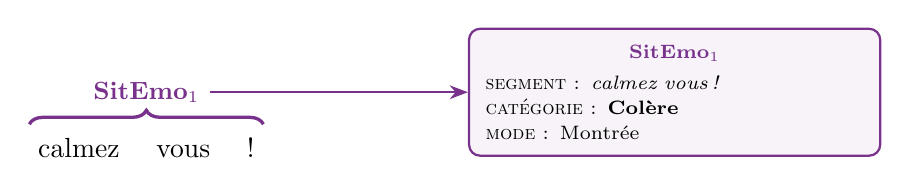
\begin{tikzpicture}[
  >=Stealth,
  word/.style={font=\normalsize, inner sep=1pt, anchor=base west},
  infobox/.style={draw=#1, thick, rounded corners=4pt, fill=#1!6,
                  inner sep=6pt, font=\scriptsize, text width=4.8cm,
                  align=left},
  brtop/.style={decorate,
                decoration={brace, amplitude=5pt, raise=4pt},
                very thick, #1}
]

% ---------- Mots de la phrase ----------
\node[word] (w1) at (-2,0)    {calmez};
\node[word] (w2) at (-0.5,0)  {vous};
\node[word] (w3) at (0.65,0)  {!};

% ---------- Accolade DESSUS : SitEmo₁ (Montrée / violet) ----------
\draw[brtop=colMontre]
  ([xshift=-2pt]w1.north west) -- ([xshift=2pt]w3.north east)
  node[midway, above=8pt, colMontre, font=\small\bfseries]
  (labse1) {SitEmo$_1$};

% ---------- Boîte d'information ----------
\coordinate (boxX) at (3.5, 0);
\node[infobox=colMontre, anchor=west] (i1) at (labse1 -| boxX) {
  \makebox[\linewidth][c]{\textcolor{colMontre}{\textbf{SitEmo$_1$}}}\\[3pt]
  \textsc{segment}~: \textit{calmez vous\,!}\\[1pt]
  \textsc{catégorie}~: \textbf{Colère}\\[1pt]
  \textsc{mode}~: Montrée
};

% ---------- Flèche reliant accolade → boîte ----------
\draw[->, thick, colMontre]
  (labse1.east) -- (i1.west);

\end{tikzpicture}

\label{fig:sans_chevauchement}
\end{figure}


Il peut y avoir un chevauchement de segments textuels associés à deux unités \texttt{SitEmo} différentes au sein d'une même phrase Par exemple, un mot peut être dans l'intersection de deux \textit{segments} des deux unités \texttt{SitEmo} différentes accolées à une même phrase comme c'est le cas ci-dessous :

% =============================================================
%  FIGURE – CHEVAUCHEMENT D'ANNOTATIONS
% =============================================================

\begin{figure}[ht]
\centering
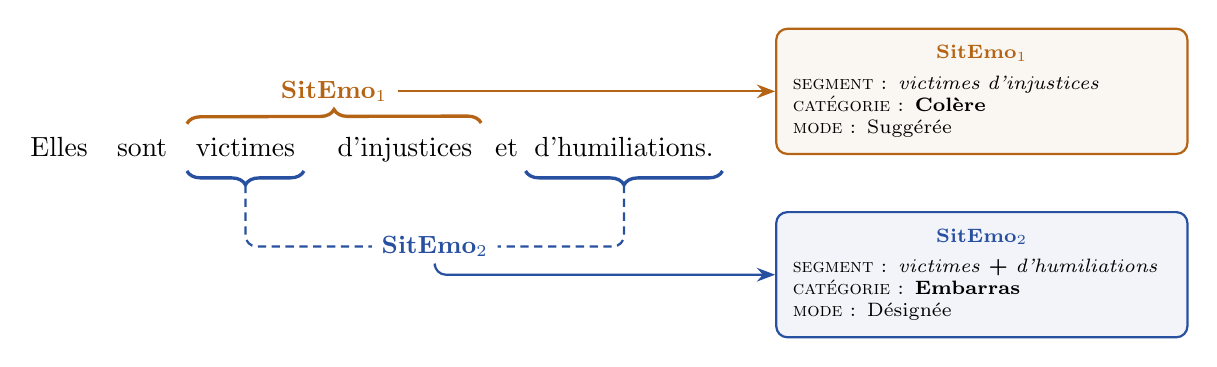
\begin{tikzpicture}[
  >=Stealth,
  word/.style={font=\normalsize, inner sep=1pt, anchor=base west},
  infobox/.style={draw=#1, thick, rounded corners=4pt, fill=#1!6,
                  inner sep=6pt, font=\scriptsize, text width=4.8cm,
                  align=left},
  brtop/.style={decorate,
                decoration={brace, amplitude=5pt, raise=4pt}, % <-- raise diminué à 4pt
                very thick, #1},
  brbot/.style={decorate,
                decoration={brace, amplitude=5pt, mirror, raise=4pt}, % <-- raise diminué à 4pt
                very thick, #1}
]

% ---------- Mots de la phrase (décalés à gauche) ----------
\node[word] (w1) at (-2,0)     {Elles};
\node[word] (w2) at (-0.9,0)   {sont};
\node[word] (w3) at (0.1,0)   {victimes};
\node[word] (w4) at (1.9,0)   {d'injustices};
\node[word] (w5) at (3.9,0)   {et};
\node[word] (w6) at (4.4,0)   {d'humiliations.};

% ---------- Accolade DESSUS : SitEmo₁ (Suggérée / ambre) ----------
\draw[brtop=colSugg]
  ([xshift=-2pt]w3.north west) -- ([xshift=2pt]w4.north east)
  node[midway, above=8pt, colSugg, font=\small\bfseries] % <-- above ajusté à 8pt
  (labse1) {SitEmo$_1$};

% ---------- Accolades DESSOUS : SitEmo₂ (Désignée / bleu) ----------
\draw[brbot=colDesigne]
  ([xshift=-2pt]w3.south west) -- ([xshift=2pt]w3.south east);
\draw[brbot=colDesigne]
  ([xshift=-2pt]w6.south west) -- ([xshift=2pt]w6.south east);
% Étiquette centrée entre les deux fragments
\node[colDesigne, font=\small\bfseries]
  (lab2) at ($(w3.south)!0.5!(w6.south) + (0,-1.1)$)
  {SitEmo$_2$};
% Lignes en pointillés (yshift ajusté à -9pt au lieu de -11pt pour coller à la pointe)
\draw[colDesigne, densely dashed, thick, rounded corners]
  ([yshift=-9pt]w3.south) |- (lab2.west);
\draw[colDesigne, densely dashed, thick, rounded corners]
  ([yshift=-9pt]w6.south) |- (lab2.east);

% ---------- Boîtes d'information ----------

% Création d'un repère d'alignement pour que les deux boîtes soient au même niveau x (7.5)
\coordinate (boxX) at (7.5, 0);

% Box SitEmo₁ (ambre) – positionnée automatiquement à la hauteur exacte de labse1
% L'opérateur (-| boxX) donne "l'ordonnée de labse1 et l'abscisse de boxX"
\node[infobox=colSugg, anchor=west] (i1) at (labse1 -| boxX) {
  \makebox[\linewidth][c]{\textcolor{colSugg}{\textbf{SitEmo$_1$}}}\\[3pt]
  \textsc{segment} : \textit{victimes d'injustices}\\
  \textsc{catégorie} : \textbf{Colère}\\
  \textsc{mode} : Suggérée
};
% Box SitEmo₂ (bleu) – placée plus bas, bien séparée
\node[infobox=colDesigne, anchor=west] (i2) at (7.5, -1.5) {
  \makebox[\linewidth][c]{\textcolor{colDesigne}{\textbf{SitEmo$_2$}}}\\[3pt]
  \textsc{segment} : \textit{victimes} \textbf{+}
                   \textit{d'humiliations}\\
  \textsc{catégorie} : \textbf{Embarras}\\
  \textsc{mode} : Désignée
};

% ---------- Flèches reliant accolades → boîtes ----------
% Flèche SitEmo₁ (ambre) : parfaitement droite horizontale maintenant
\draw[->, thick, colSugg]
  (labse1.east) -- (i1.west);
% Flèche SitEmo₂ (bleu) : part d'en dessous de SitEmo2, descend puis tourne
\draw[->, thick, colDesigne, rounded corners=4pt]
  (lab2.south) |- (i2.west);

\end{tikzpicture}
\label{fig:chevauchement}
\end{figure}


% =============================================================
%  TRANSITION VERS LE NIVEAU VECTORIEL
% =============================================================




\newpage

\subsection*{Des annotations linguistiques à leurs représentations vectorielles}

\begin{figure}[ht]
\centering
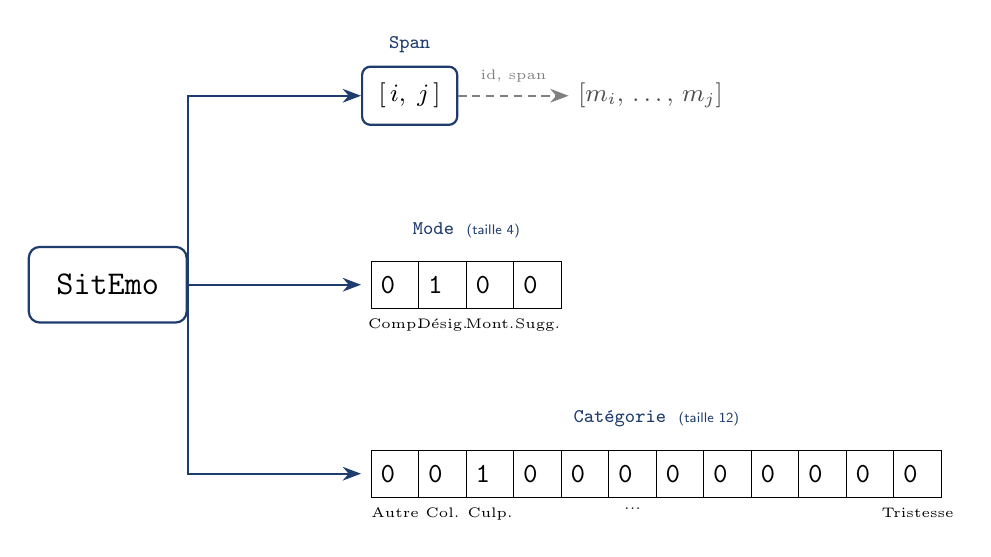
\begin{tikzpicture}[
    >=Stealth,
    node distance=2cm,
    vector/.style={
        matrix of nodes,
        nodes={draw, minimum size=6mm, anchor=center, align=center,
               font=\ttfamily},
        column sep=-\pgflinewidth,
        row sep=-\pgflinewidth,
        nodes in empty cells
    },
    labelbox/.style={font=\sffamily\scriptsize, text=bleufonce, align=center}
]

% --- Noeud central SitEmo ---
\node[draw=bleufonce, thick, rounded corners,
      inner sep=10pt, font=\large\ttfamily] (sitemo) {SitEmo};

% ============================================================
%  SPAN  (paire d'indices — en haut)
% ============================================================
\node[draw=bleufonce, thick, rounded corners=3pt,
      inner sep=6pt, font=\small\ttfamily,
      right=2.2cm of sitemo, yshift=2.4cm] (span) {%
    $[\,i,\; j\,]$%
};
\node[labelbox, above=1pt of span] {\texttt{Span}};

% --- Segment textuel (résultat du lookup) ---
\node[right=1.4cm of span, font=\small\itshape,
      text=black!70, align=left] (seg) {%
    $[m_i,\,\ldots,\,m_j]$};
\draw[->, densely dashed, black!50, thick]
    (span.east) -- (seg.west)
    node[midway, above=1pt, font=\tiny, text=black!50] {id, span};

% ============================================================
%  MODE  (vecteur binaire de taille 4 — au milieu)
% ============================================================
\matrix[vector, right=2.2cm of sitemo] (mode) {
    0 & 1 & 0 & 0 \\
};
\node[labelbox, above=1pt of mode] {\texttt{Mode}\; {\tiny(taille 4)}};
\node[font=\tiny, anchor=north] at (mode-1-1.south) {Comp.};
\node[font=\tiny, anchor=north] at (mode-1-2.south) {Désig.};
\node[font=\tiny, anchor=north] at (mode-1-3.south) {Mont.};
\node[font=\tiny, anchor=north] at (mode-1-4.south) {Sugg.};

% ============================================================
%  CATÉGORIE  (vecteur binaire de taille 12 — en bas)
% ============================================================
\matrix[vector, right=2.2cm of sitemo, yshift=-2.4cm] (cat) {
    0 & 0 & 1 & 0 & 0 & 0 & 0 & 0 & 0 & 0 & 0 & 0 \\
};
\node[labelbox, above=1pt of cat] {\texttt{Catégorie}\; {\tiny(taille 12)}};
\node[font=\tiny, anchor=north] at (cat-1-1.south)  {Autre};
\node[font=\tiny, anchor=north] at (cat-1-2.south)  {Col.};
\node[font=\tiny, anchor=north] at (cat-1-3.south)  {Culp.};
\node[font=\tiny, anchor=north] at (cat-1-6.south)  {...};
\node[font=\tiny, anchor=north] at (cat-1-12.south) {Tristesse};

% ============================================================
%  FLÈCHES depuis SitEmo
% ============================================================
\draw[->, thick, bleufonce] (sitemo.east) |- (span.west);
\draw[->, thick, bleufonce] (sitemo.east) -- (mode.west);
\draw[->, thick, bleufonce] (sitemo.east) |- (cat.west);

\end{tikzpicture}
\caption{Représentation d'une unité \texttt{SitEmo} comme triplet
         {\fontfamily{phv}\selectfont\small (Span\,; Catégorie\,; Mode)}.
         La flèche en pointillés indique que la récupération du segment
         textuel nécessite à la fois le \texttt{Span} et un identifiant
         de la phrase source.}
\label{fig:vecteurs_sitemo}
\end{figure}


Les deux traits peuvent être représentés par des vecteurs de taille~4 et de taille~12
respectivement, sur lesquels il n'y a que des 1 ou des 0 qui indiquent
la présence ou l'absence de l'attribut correspondant.

On peut présenter de manière simplifiée ce qu'est la représentation vectorielle d'une unité
\texttt{SitEmo} dans le schéma d'annotation de \textcite{etienne2023} comme un triplet~:
\[
(\texttt{span}_{X},\; \texttt{émotion}_{Y},\; \texttt{mode}_{Z})
\]
où $\texttt{span}_{X}$ désigne un intervalle textuel, $\texttt{émotion}_{Y}$ est un vecteur de taille~12 indiquant la catégorie émotionnelle~$Y$, et $\texttt{mode}_{Z}$ est un vecteur \textit{one-hot} de taille~4 indiquant le mode d'expression~$Z$. Ce triplet signifie que l'émotion~$Y$ est réalisée selon le mode~$Z$ sur le segment textuel associé au~$\texttt{span}_{X}$\footnote{Nous supposons qu'il n'y a qu'une seule catégorie émotionnelle par soucis de simplicité, mais dans le schéma d'annotation de \textcite{etienne2023} si on ne compte pas l'indice qui correspond à "autre", le vecteur peut avoir jusqu'à deux indices activés simultanément, et jusqu'à trois si on le compte}.

\newpage
\subsection*{Ajout de l'étiquette \texttt{type} à partir des précédentes annotations}

À partir de ces annotations préalables réalisées avec un grain assez fin, il est possible d'assigner de nouvelles étiquettes avec un grain plus épais. À chaque unité \texttt{SitEmo}, on peut ajouter un type :

% ---------- Figure Base / Complexe / Autre ----------
\begin{figure}[ht]
\centering
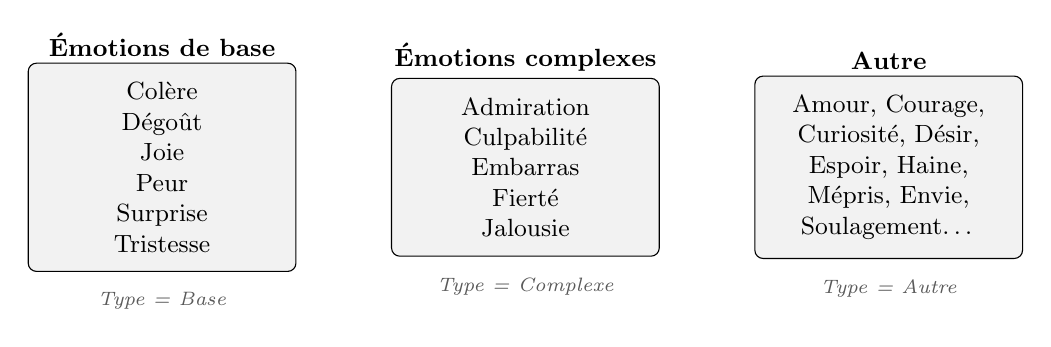
\begin{tikzpicture}[
  catbox/.style={draw, rectangle, rounded corners=3pt, align=center,
                 inner sep=7pt, font=\small, minimum width=3.4cm, fill=gray!10},
  titre/.style={font=\small\bfseries, fill=white, inner sep=2pt},
  sous/.style={font=\scriptsize\itshape, text=black!65, align=center}
]

\node[catbox] (base) {
  Colère \\ Dégoût \\ Joie \\ Peur \\ Surprise \\ Tristesse
};
\node[titre, anchor=south] (t1) at (base.north) {Émotions de base};
\node[sous, below=4pt of base] (s1) {Type = Base};

\node[catbox, right=1.2cm of base] (complex) {
  Admiration \\ Culpabilité \\ Embarras \\ Fierté \\ Jalousie
};
\node[titre, anchor=south] (t2) at (complex.north) {Émotions complexes};
\node[sous, below=4pt of complex] (s2) {Type = Complexe};

\node[catbox, right=1.2cm of complex] (other) {
  Amour, Courage,\\ Curiosité, Désir,\\
  Espoir, Haine,\\ Mépris, Envie,\\
  Soulagement\ldots
};
\node[titre, anchor=south] at (other.north) {Autre};
\node[sous, below=4pt of other] {Type = Autre};

\end{tikzpicture}
\caption{Les trois types d'émotions.}
\end{figure}

\subsubsection*{Transposition des annotations qui s'ancrent sur les segments de taille variables à des annotations qui s'ancrent sur les phrases entières}

Les annotations décrites ci-dessus portent sur des \emph{segments textuels} souvent infraphrasiques.  

Arrivé ici, une phrase peut être associée à \textit{aucune} unité \texttt{SitEmo}, à une unité \texttt{SitEmo}, ou à plusieurs unités \texttt{SitEmo}. 
Arrivé ici, une unité \texttt{SitEmo} a la forme {\fontfamily{phv}\selectfont\small (Span ; Catégorie ; Mode ; Type)}. 

Le dataset manque d'uniformité pour l'entraînement d'un modèle : certaines phrases très denses sont associés à beaucoup de vecteurs, et d'autres, pauvres en expression émotionnelle, sont associées à rien du tout.

C'est l'une des raisons pour lesquelles \textcite{etienne2023} n'entraîne pas \textsc{Emotyc} sur ces
annotations locales à grain fin, mais sur une version agrégée au niveau
de la phrase.
Elle opte plus précisément pour une classification globale à l'échelle de la phrase entière. Pour cela, elle procède à une "transposition" ou "agrégation" des annotations locales. L'avantage est un gain de simplicité et une uniformisation, un inconvénient est que cela fait perdre le lien explicite entre une émotion donnée et son mode d'expression. Pour les phrases sémantiquement denses, où coexistent plusieurs annotations distinctes, la solidarité entre étiquette émotionnelle et étiquette de mode est rompue.

Il s'agit d'associer à chaque phrase \textcite[p.~135]{etienne2023} un vecteur dont chaque valeur indique l'appartenance ou non à 19~classes binaires\footnote{Les \textit{gold labels} consistent \og en une liste de 19~booléens toujours ordonnée de la même
manière, où chaque booléen renvoie à une classe et indique si elle est
présente ou non~\fg{}}. Chaque classe correspond à un prédicat binaire appliqué à la phrase.
Chaque label $y_k$ est une fonction indicatrice de la forme~:
\[
y_k(s_j) =
\begin{cases}
1 & \text{si } \varphi_k(s_j), \\
0 & \text{sinon,}
\end{cases}
\]




Le passage des annotations fines aux labels de classification consiste
donc en un \emph{transfert}~: dès qu'un segment de la phrase porte une
propriété, le label correspondant est activé pour la phrase entière. Le
modèle \textsc{Emotyc} perd de ce fait le caractère ``infraphrasique'',
passant d'annotations au niveau de granularité des mots à des
annotations au niveau des phrases.

Le but de cette transposition est de tester ou d'entraîner le modèle de classification \textsc{Emotyc}, qui opère au niveau de la \emph{phrase}\footnote{Pour être rigoureux, l'entrée $s_j$
peut prendre deux formes
\parencite[p.~105]{etienne2023}~: soit la phrase isolée, soit la phrase
encadrée de son contexte
(\texttt{before:~\dots\ </s> current:~\dots\ </s> after:~\dots}), la
phrase avec le contexte donnant, selon
\textcite[p.149]{etienne2023} dit que l'entrée avec contexte offre de
meilleurs résultats que l'entrée phrase isolée.}.

% ---------- Vecteur 19 labels ----------

En concaténant le caractère émotionnel, le mode, le type et les
catégories émotionnelles, on obtient exactement les vecteurs utilisés
comme \textit{gold-labels} lors de l'affinage d'\textsc{Emotyc}. On peut
exprimer ``Présence émotionnelle + Mode comportemental + émotion de
base + Joie'' avec le vecteur suivant :

\begin{center}
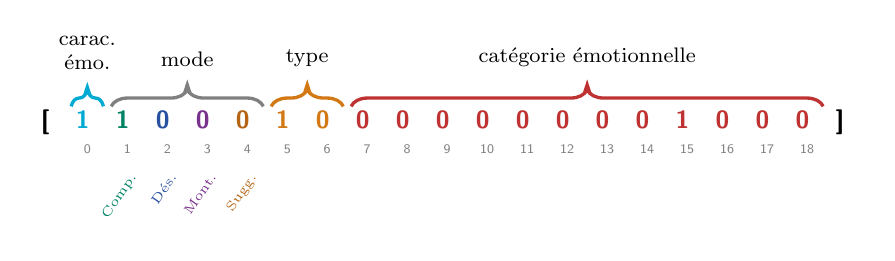
\begin{tikzpicture}[
    scale=0.95,
    transform shape,
    font=\sffamily\bfseries\small,
    brace_style/.style={decorate,
      decoration={brace, amplitude=6pt}, very thick},
    label_style/.style={font=\rmfamily\small, text=black},
    arrow_style/.style={line width=0.9pt, line cap=round,
      shorten <=1.2mm, -{Stealth[length=2.2mm,width=1.4mm]}}
]
    % --- Matrice du vecteur ---
    \matrix (vec) [
        matrix of nodes,
        nodes in empty cells,
        column sep=0.32em,
        nodes={inner sep=1.5pt, align=center}
    ] {
        {[} &
        % 0: Emo
        \textcolor{mycyan}{1} &
        % 1–4: Comp, Dés, Mont, Sugg
        \textcolor{colComp}{1} &
        \textcolor{colDesigne}{0} &
        \textcolor{colMontre}{0} &
        \textcolor{colSugg}{0} &
        % 5–6: Base, Complexe
        \textcolor{myorange}{1} &
        \textcolor{myorange}{0} &
        % 7–18: Adm, Aut, Col, Culp, Dég, Emb, Fier, Jal, Joie, Peur, Surp, Trist
        \textcolor{myred}{0} &
        \textcolor{myred}{0} &
        \textcolor{myred}{0} &
        \textcolor{myred}{0} &
        \textcolor{myred}{0} &
        \textcolor{myred}{0} &
        \textcolor{myred}{0} &
        \textcolor{myred}{0} &
        \textcolor{myred}{1} &
        \textcolor{myred}{0} &
        \textcolor{myred}{0} &
        \textcolor{myred}{0} &
        {]} \\
    };

    % --- Indices sous chaque cellule ---
    \foreach \i/\lab in {
      2/{\tiny 0},3/{\tiny 1},4/{\tiny 2},5/{\tiny 3},6/{\tiny 4},
      7/{\tiny 5},8/{\tiny 6},
      9/{\tiny 7},10/{\tiny 8},11/{\tiny 9},12/{\tiny 10},
      13/{\tiny 11},14/{\tiny 12},15/{\tiny 13},16/{\tiny 14},
      17/{\tiny 15},18/{\tiny 16},19/{\tiny 17},20/{\tiny 18}}{
      \node[below=1pt of vec-1-\i, font=\sffamily, text=black!50] {\lab};
    }

    % --- Accolades supérieures ---
    % Emo
    \draw[brace_style, mycyan]
        (vec-1-2.north west) -- (vec-1-2.north east)
        coordinate[midway] (c1);
    \draw[arrow_style, mycyan]
        ([yshift=3.1pt]c1) -- ++(0,0.22)
        node[above=1pt, label_style, align=center]
        {\footnotesize carac.\\[-2pt]\footnotesize émo.};

    % Mode (indices 1–4, chaque cellule dans la couleur de son mode)
    \draw[brace_style, black!50]
        (vec-1-3.north west) -- (vec-1-6.north east)
        coordinate[midway] (c2);
    \draw[arrow_style, black!50]
        ([yshift=4pt]c2) -- ++(0,0.22)
        node[above=1pt, label_style] {\footnotesize mode};

    % Type
    \draw[brace_style, myorange]
        (vec-1-7.north west) -- (vec-1-8.north east)
        coordinate[midway] (c3);
    \draw[arrow_style, myorange]
        ([yshift=4pt]c3) -- ++(0,0.22)
        node[above=1pt, label_style] {\footnotesize type};

    % Catégorie
    \draw[brace_style, myred]
        (vec-1-9.north west) -- (vec-1-20.north east)
        coordinate[midway] (c4);
    \draw[arrow_style, myred]
        ([yshift=4pt]c4) -- ++(0,0.22)
        node[above=1pt, label_style]
        {\footnotesize catégorie émotionnelle};

    % --- Noms des labels sous les indices ---
    \node[below=10pt of vec-1-3, font=\tiny, colComp, rotate=55,
          anchor=north east] {Comp.};
    \node[below=10pt of vec-1-4, font=\tiny, colDesigne, rotate=55,
          anchor=north east] {Dés.};
    \node[below=10pt of vec-1-5, font=\tiny, colMontre, rotate=55,
          anchor=north east] {Mont.};
    \node[below=10pt of vec-1-6, font=\tiny, colSugg, rotate=55,
          anchor=north east] {Sugg.};

\end{tikzpicture}
\end{center}
\newpage

\appendix

\section*{Annexe 1}

\begin{tabular}{@{} >{\bfseries}l p{10cm} @{}}
\toprule
Catégorie & Émotions fines associées \\
\midrule
Colère & agacement, colère, contestation, désaccord (en suggérée),
         désapprobation, énervement, fureur/rage, indignation,
         insatisfaction, irritation, mécontentement, réprobation,
         révolte \\
Dégoût & dégoût, lassitude, répulsion \\
Joie   & amusement, enthousiasme, exaltation, joie, plaisir \\
Peur   & angoisse, appréhension, effroi, horreur, inquiétude,
         méfiance, peur, stress, timidité\textsuperscript{*} \\
Surprise  & étonnement, stupeur, surprise \\
Tristesse & blues, chagrin, déception, désespoir, peine, souffrance,
            tristesse \\
\addlinespace
Admiration  & admiration \\
Culpabilité & culpabilité \\
Embarras    & embarras, gêne, honte, humiliation,
              timidité\textsuperscript{*} \\
Fierté      & fierté, orgueil \\
Jalousie    & jalousie \\
\addlinespace
Autre & amour, courage, curiosité, désir, détermination, envie,
        espoir, haine, impuissance, mépris, soulagement \\
\bottomrule
\end{tabular}

\smallskip
\noindent{\footnotesize \textsuperscript{*}\,\emph{Timidité} appartient
à la fois à \textsc{Peur} et à \textsc{Embarras}.}


\vspace{10mm}
Remarque : ce tableau ne permet pas de rendre compte des \textit{similarités} et
des éventuels chevauchements, il conviendrait bien plutôt de délimiter
spatialement, dans un espace de très haute dimensionalité, l'extension
associée à chacune de ces émotions, puis à faire des réductions de
dimensionalité, afin d'avoir une classification donnant à voir (en 2D ou
3D) les similarités (resp.\ dissimilarités) par les proximités
(resp.\ éloignements).
\printbibliography

\end{document}
